\section{Part A}
\subsection{Technical Discussion}
Figure \ref{fig:original} shows a magnetic resonance image(MRI) of an upper thoracic human spine with a facture dislocation and spinal cord impingement. Because the original image is predominantly dark, an expansion of intensity levels is desirable. This can be accomplished with Log Transformation and Power-Low(Gamma) Transformation.
\begin{figure}[h]
\centering
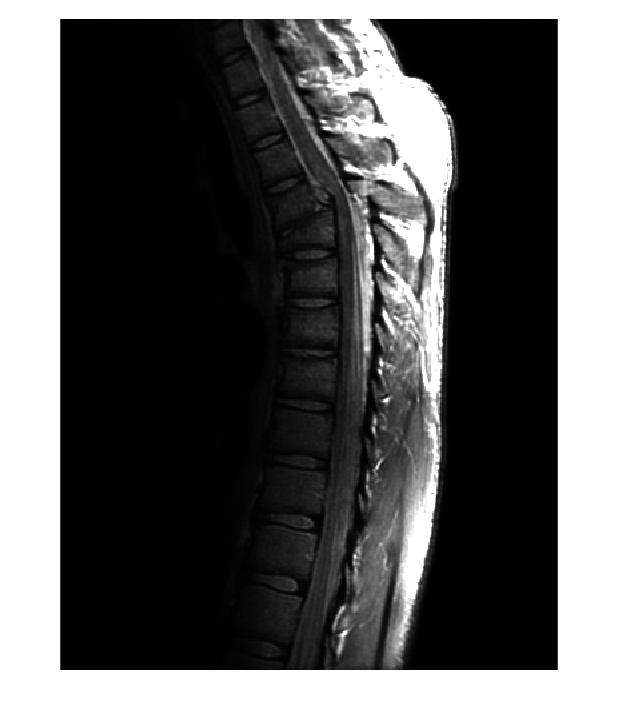
\includegraphics[scale=0.2]{0308}
\caption{Original Image}
\label{fig:original}
\end{figure}
\subsubsection{Log Transformations}
The general form of the log transformation is
$$ s=clog(1 + r) $$
where $r$ is the original pixel value between 0 and 1, $s$ is the pixel value after log transformation and $c$ is a constant. By observing the function we could find that this transformation maps a narrow range of low intensity values in the input into a wider range of output levels. We could use this kind of transformation to expand the values of dark pixels in the given MRI and compressing the higher-level values, which could show the details of the fractured part more obvious. 
\subsubsection{Power-Law(Gamma) Transformations}
Power-law transformations have the basic form
$$ s = cr^{\gamma} $$
Where where $r$ is the original pixel value between 0 and 1 and $s$ is the pixel value after transformation. $c$ and $ \gamma $ are positive constants. By observing the equation we could find that power-law transformation also map a narrow range of dark input values into a wider range of output values. By analyzing, we could notice that when $\gamma > 1$, the produced image tend to be darker than the original image. However, when $\gamma < 1$, the produced image will show more details on dark area of original image. In the following experiments, we need to find appropriate $c$ and $\gamma$ to show more details of the given MRI.
\subsection{Discussion of Results}
\subsubsection{Experiments of Log Transformations}
The experiments results of log transformation shows below:
\begin{figure}[h]
	\centering
	\subfloat[Subfigure 1 list of figures text][Original Image]{
		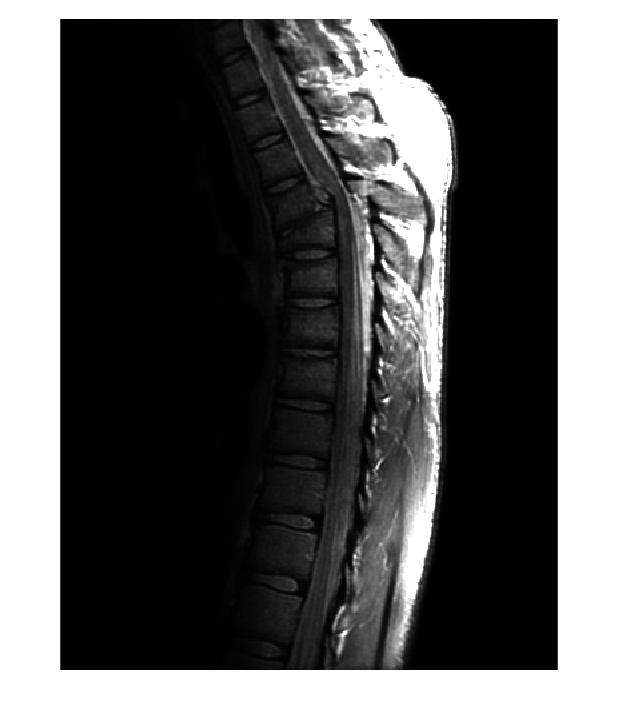
\includegraphics[width=0.2\textwidth]{0308}
		\label{fig:subfig1}}
	\subfloat[Subfigure 2 list of figures text][$c=1$]{
		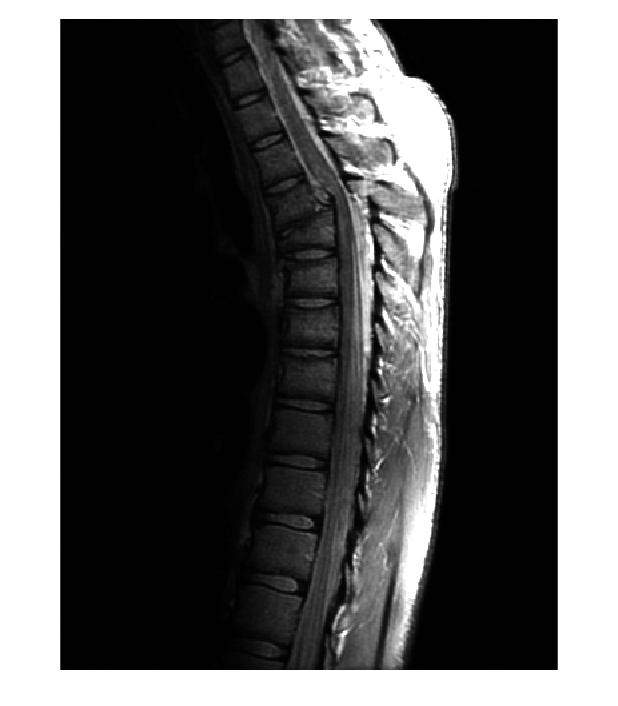
\includegraphics[width=0.2\textwidth]{logc1}
		\label{fig:subfig2}}
	\subfloat[Subfigure 3 list of figures text][$c=3$]{
		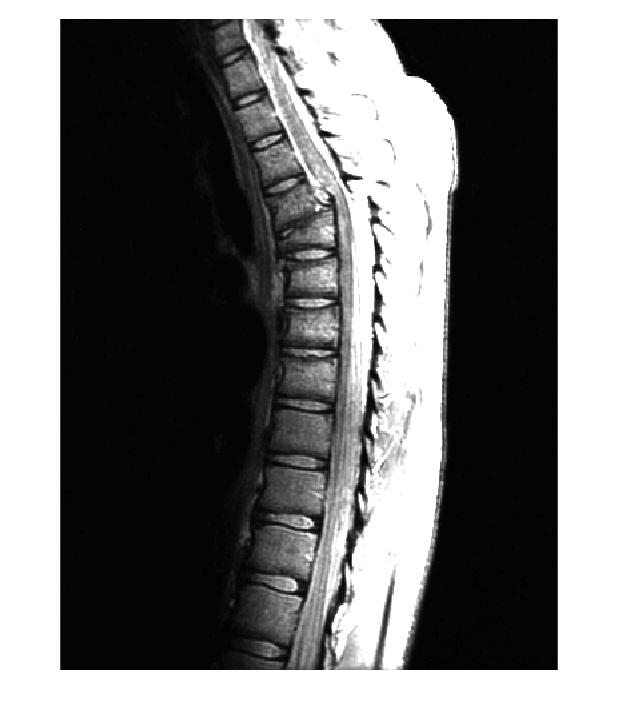
\includegraphics[width=0.2\textwidth]{logc3}
		\label{fig:subfig3}}
	\subfloat[Subfigure 4 list of figures text][$c=6$]{
		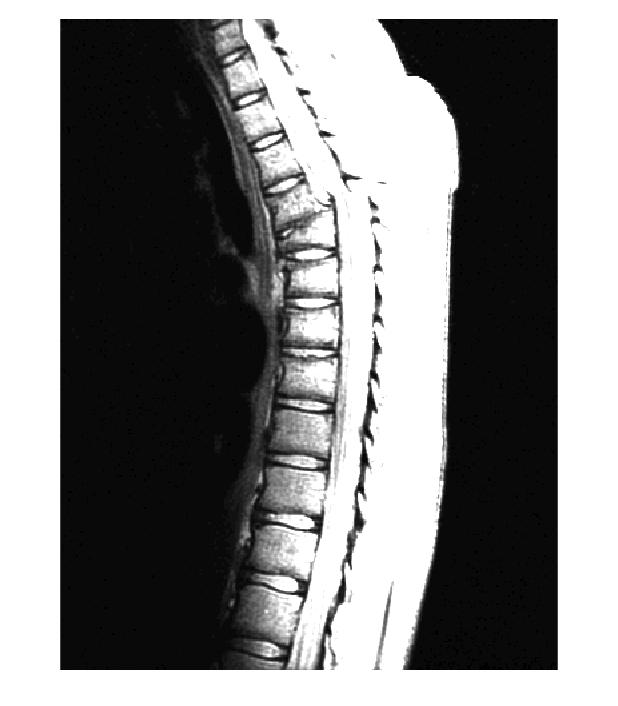
\includegraphics[width=0.2\textwidth]{logc6}
		\label{fig:subfig4}}
	\caption{Experiments results of log transformation when $c=$ 1, 3 and 6}
	\label{fig:exlogfig}	
\end{figure}
As shown in Figure \ref{fig:subfig2}, the produced image shows more details on the dark area compare with the given MRI. However, the fractured area on the dark side still not clear enough. When we have $c=6$, we could find even more details on the dark area as it shows in Figure \ref{fig:subfig4}. But we could also notice that those area around the fractured point become totally white, which may result in missing of important information. As shown in Figure \ref{fig:subfig3} When $c=3$, we could have a relative desirable output image since it provides us enough information about the fracture also dark area. \par
\begin{figure}[h]
	\centering
	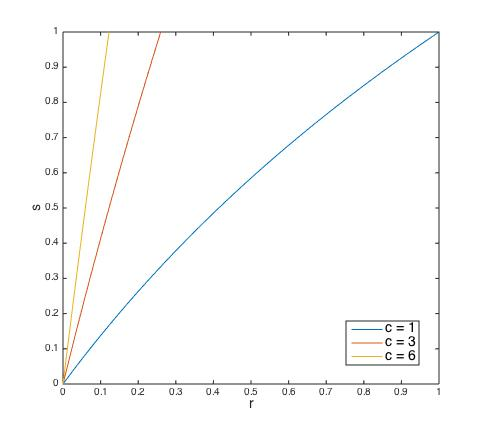
\includegraphics[scale=0.4]{log136}
	\caption{The curve of $clog(r + 1)$ when $c =$ 1, 3 and 6}
	\label{fig:curvelog}
\end{figure}

The reason behind it could be found in Figure \ref{fig:curvelog}. As shown in the figure, we could notice that when $c = 1$ the output pixel value $s$ just grow a little compare with original value $r$. This is why it shows a little bit more details but the fractured area is still not clear enough. We note that, as $c$ increased to 3, the output pixel grows much higher than the original pixel value. So the produced image shows more details compare with $c = 1$. According to the curve above, $s$ will equal to 1 when $r > 0.26$, which may result in missing some information but still at an acceptable level. However, as $c$ increase from 3 to 6, although we could have more details on the darker area, any input pixel value $r > 0.11$ will map to 1 according to the curve. It means we will miss lots of detail informations on the lighter side of image by selecting $c = 6$. So, when $c = 3$ the output image could have best visual enhancement.
\subsubsection{Experiments of Power-Law Transformations}
The experiments results of Power-Law(gamma) transformation shows in Figure \ref{fig:powerfig}.\\
\\
Since the basic form of Power-law transformations is
$$ s = cr^{\gamma} $$
By selecting $c$ and $\gamma$, we can get the optimal parameters with best visual result.\\
\\
As shown in \ref{fig:psubfig2}, when $c = 1$ and $\gamma=1.5$, the produced image is darker than original image and area near fractured point became invisible. With $ c = 1$ and $\gamma$ decreased from 0.8 to 0.4 as shown in Figure \ref{fig:psubfig3}, \ref{fig:psubfig4}, \ref{fig:psubfig5}, more detaild became visible. As shown in Figure \ref{fig:psubfig6} A further decrease of $\gamma$ to 0.3 enhanced a little more detail in background but begin to reduce contrast to the point where the image started to have a slight washed-out appearance. If we decreased $c$ to 0.5 and let $\gamma = 0.4$, the produced image became much darker than original image as shown in \ref{fig:psubfig7}. Similarly, As shown in Figure \ref{fig:psubfig8}, if $c = 1.5$ and $\gamma = 0.4$, although the produced image shows more details on the dark side compare with original image, image on the lighter side became totally white and missing some details. By comparing all results, produced image will have best visual result with $c = 1$ and $\gamma = 0.4$. 

\begin{figure}[h]
	\centering
	\subfloat[Subfigure 1 list of figures text][Original Image]{
		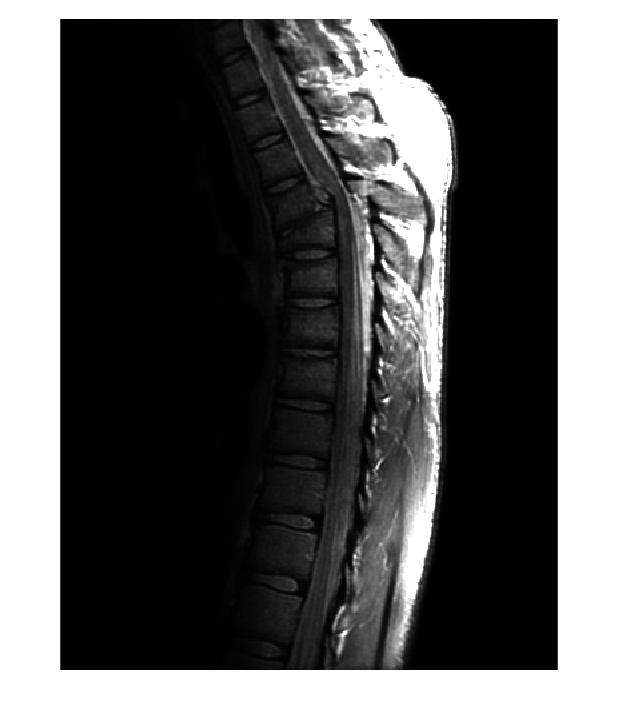
\includegraphics[width=0.2\textwidth]{0308}
		\label{fig:psubfig1}}
	\subfloat[Subfigure 2 list of figures text][$c=1, \gamma=1.5$]{
		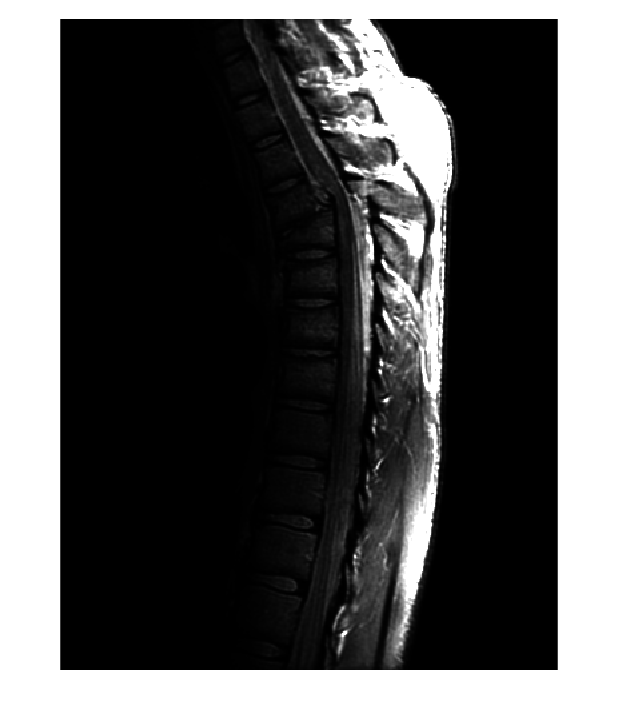
\includegraphics[width=0.2\textwidth]{c1r1_5}
		\label{fig:psubfig2}}
	\subfloat[Subfigure 3 list of figures text][$c=1, \gamma=0.8$]{
		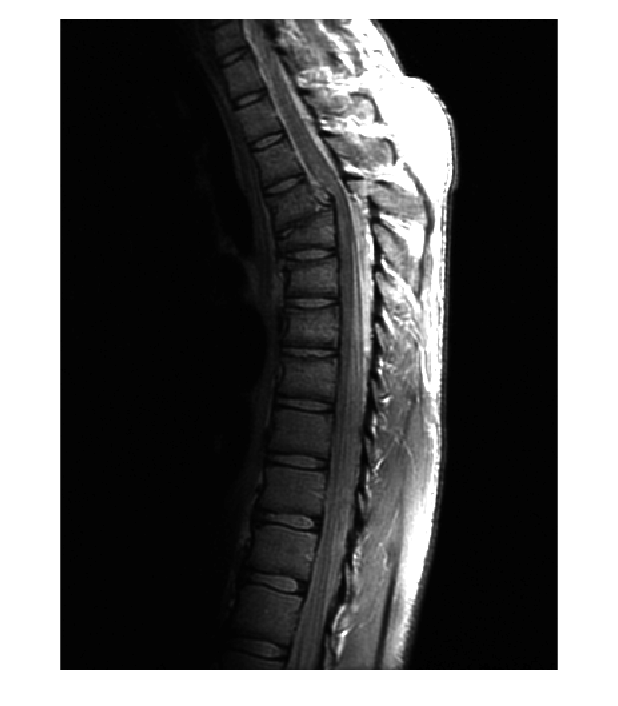
\includegraphics[width=0.2\textwidth]{c1r0_8}
		\label{fig:psubfig3}}
	\subfloat[Subfigure 4 list of figures text][$c=1, \gamma=0.5$]{
		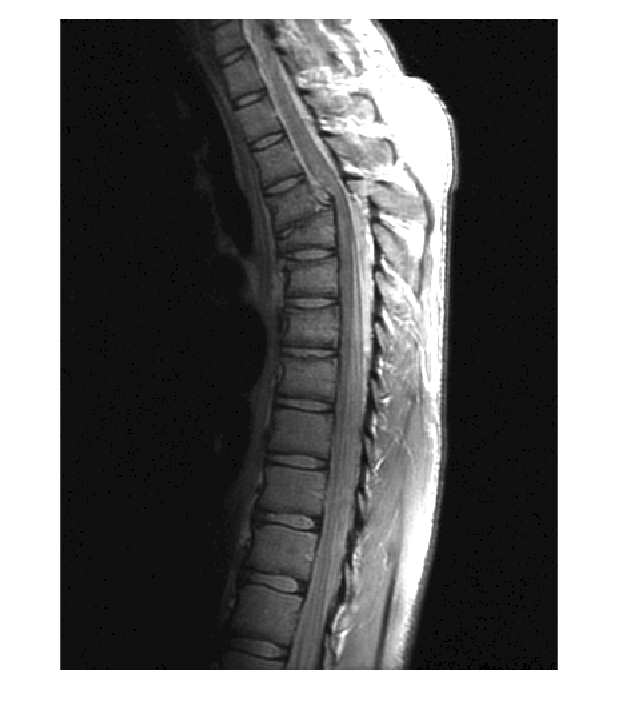
\includegraphics[width=0.2\textwidth]{c1r0_5}
		\label{fig:psubfig4}}\\
	\subfloat[Subfigure 5 list of figures text][$c=1, \gamma=0.4$]{
		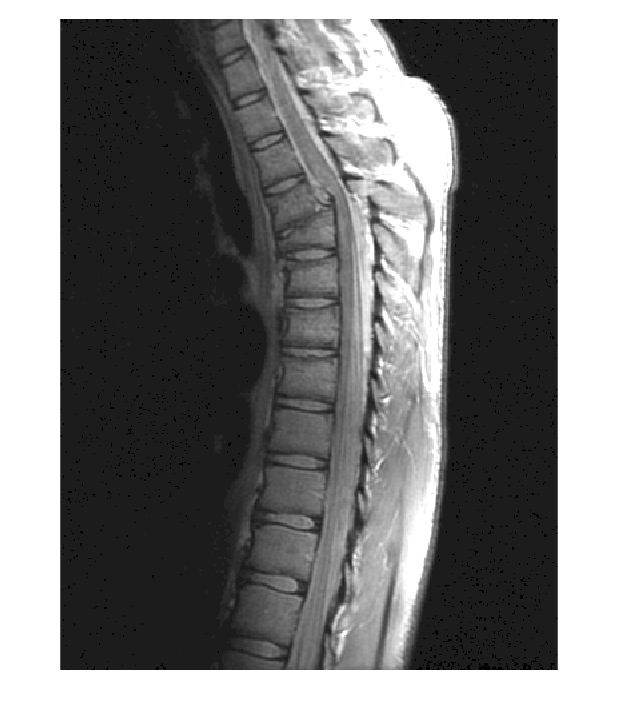
\includegraphics[width=0.2\textwidth]{c1r0_4}
		\label{fig:psubfig5}}
	\subfloat[Subfigure 6 list of figures text][$c=1, \gamma=0.3$]{
		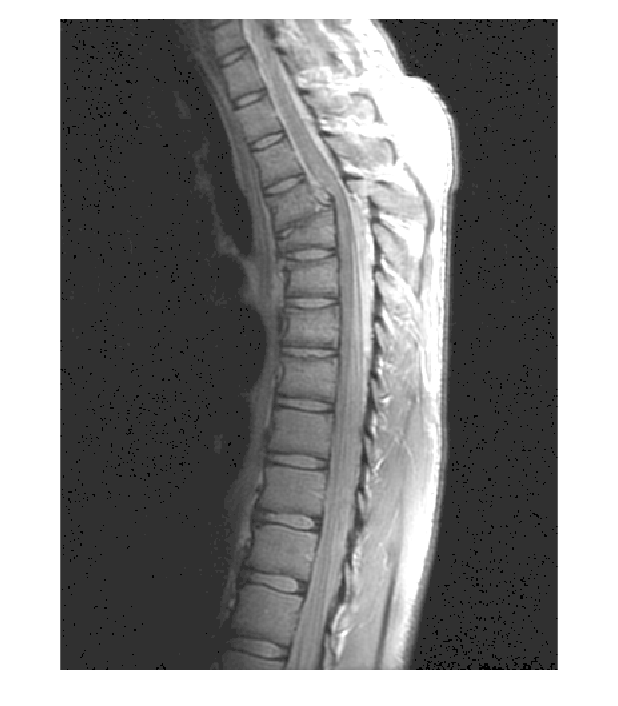
\includegraphics[width=0.2\textwidth]{c1r0_3}
		\label{fig:psubfig6}}
	\subfloat[Subfigure 7 list of figures text][$c=0.5, \gamma=0.4$]{
		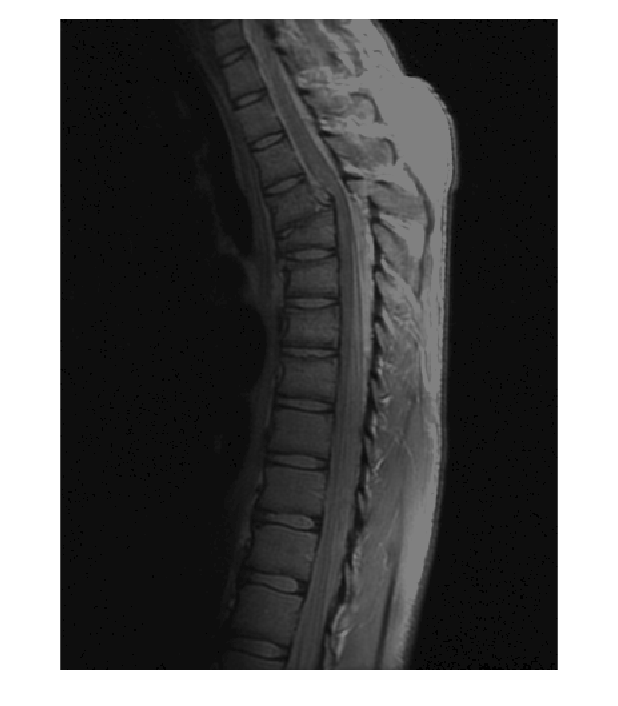
\includegraphics[width=0.2\textwidth]{c0_5r0_4}
		\label{fig:psubfig7}}
	\subfloat[Subfigure 8 list of figures text][$c=1.5, \gamma=0.4$]{
		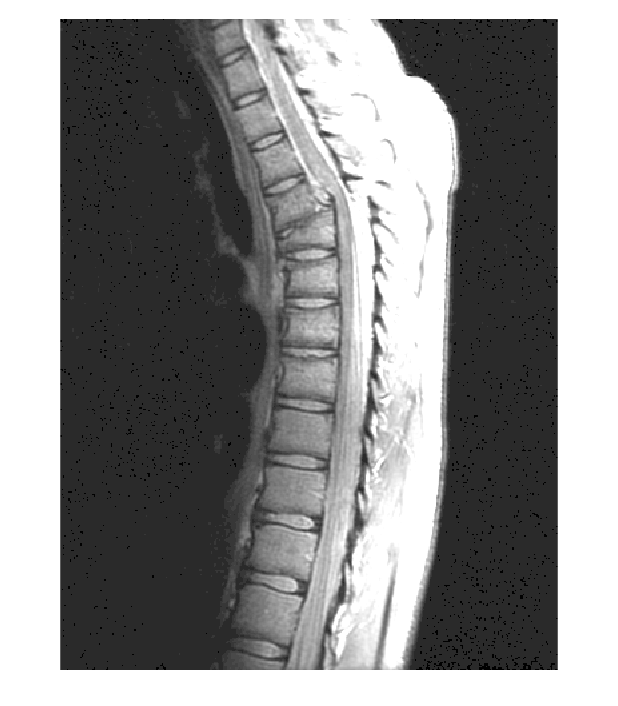
\includegraphics[width=0.2\textwidth]{c1_5r0_4}
		\label{fig:psubfig8}}
	\caption{Experiments results of Power-Law transformation}
	\label{fig:powerfig}
\end{figure}
\par
\begin{figure}[h]
	\centering
	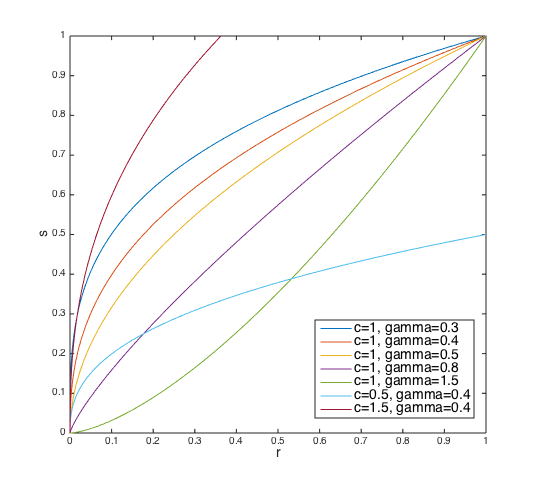
\includegraphics[scale=0.3]{powercr}
	\caption{The curve of $s = cr^{\gamma}$}
	\label{fig:curvepower}
\end{figure}
The reason behind it could be found in Figure \ref{fig:curvepower}. As shown in the figure, we could notice that with $c = 1$ and $\gamma$ decreased from 0.8 to 0.3, output pixel value $s$ will grow more compare with the original input pixel value $r$. When $\gamma=0.3$, we can note that the output pixel value will become around 0.5 even the input pixel value just around 0.1. This is the reason why it begin to reduce contrast to the point where the image started to have a slight washed-out appearance. When $c = 0.5$, the output value will in a range from 0 to 0.5. So, it makes the produced image darker than original image. Similarly, If we set $c = 1.5$, we could note that when input pixel value $r \geq 0.4$, the output pixel value will be 1. So the lighter side of the produced image became white. So, when $c = 1$ and $\gamma = 0.4$ the output image could have best visual enhancement.


